\documentclass{llncs}

% ── Packages ──────────────────────────────────────────────────────────────────
\usepackage{graphicx}
\usepackage{amsmath}
\usepackage{amssymb}
\usepackage{booktabs}
\usepackage{float}
\usepackage[section]{placeins}
\usepackage{microtype}
\usepackage{xcolor}
\usepackage[colorlinks=true,linkcolor=blue!60!black,
            citecolor=blue!60!black,urlcolor=blue!60!black]{hyperref}

% Improve float placement for many figures and tables
\setcounter{topnumber}{5}
\setcounter{bottomnumber}{5}
\setcounter{totalnumber}{10}
\renewcommand{\topfraction}{0.9}
\renewcommand{\bottomfraction}{0.9}
\renewcommand{\textfraction}{0.1}
\renewcommand{\floatpagefraction}{0.8}
\renewcommand{\dbltopfraction}{0.9}
\renewcommand{\dblfloatpagefraction}{0.8}

% ── Macros for filenames containing % ─────────────────────────────────────────
\begingroup
\catcode`\%=12\relax
\gdef\imgVAEtwenty{prints/VAR20%imagens.png}
\gdef\imgGANtwenty{prints/Gan20%imagens.png}
\gdef\imgDDPMtwenty{prints/DDPM20%imagens.png}
\gdef\imgLossVAEtwenty{prints/lossGraphVAE20%.png}
\gdef\imgLossGANtwenty{prints/lossGraphGan20%.png}
\gdef\imgLossDDPMtwenty{prints/lossGraphDDPM20%.png}
\gdef\imgVAEhundred{VAEimagens100%.png}
\gdef\imgGANhundred{prints/GAN100%imagens.png}
\gdef\imgDDPMhundred{prints/DDPM100%imagens.png}
\gdef\imgLossVAEhundred{lossGraphVAE100%.png}
\gdef\imgLossGANhundred{prints/lossGraphGan100%.png}
\gdef\imgLossDDPMhundred{prints/lossGraphDDPM100%.png}
\gdef\imgMetricsHundred{analiseMetricas100%.png}
\endgroup

% ─────────────────────────────────────────────────────────────────────────────
\begin{document}

\title{Comparison of Generative Models\texorpdfstring{\\}{ }on the ArtBench-10 Dataset}

\author{Francisco Vieira Monteiro de Queiros\inst{1} \and
        Tomás Pinto Loureiro\inst{1}}

\authorrunning{F.\,V.\,M. Queiros and T.\,P. Loureiro}

\institute{University of Coimbra, Coimbra, Portugal}

\maketitle

% ══ ABSTRACT ══════════════════════════════════════════════════════════════════
\begin{abstract}
This paper presents the implementation and comparative evaluation of three
generative image model families --- a Variational Autoencoder (VAE), a Deep
Convolutional Generative Adversarial Network (DCGAN), and a Denoising
Diffusion Probabilistic Model (DDPM) --- trained on the ArtBench-10 dataset
($32\times32$ pixels, 10 artistic styles). Following a two-phase protocol,
all models were first developed and evaluated on a 20\% data subset, then
retrained on the full 50,000-image dataset. Quantitative evaluation uses
Fr\'echet Inception Distance (FID) and Kernel Inception Distance (KID),
reported as mean~$\pm$~std over 10 seeds (5,000 samples each). On the full
dataset, the DCGAN achieved the best results
(FID~$=30.46\pm0.57$; KID~$=0.0032\pm0.0001$), followed by the DDPM
(FID~$=37.91\pm0.37$; KID~$=0.0062\pm0.0002$) and the VAE
(FID~$=140.37\pm0.43$; KID~$=0.0314\pm0.0004$).

\keywords{Generative Models \and VAE \and DCGAN \and DDPM \and ArtBench-10
          \and FID \and KID}
\end{abstract}

% ══ 1. INTRODUCTION ═══════════════════════════════════════════════════════════
\section{Introduction}

Generative modelling of images has become a central research area, with
applications ranging from data augmentation to creative content synthesis.
Three paradigms have emerged as dominant: Variational Autoencoders
(VAE)~\cite{kingma2013}, Generative Adversarial Networks~\cite{radford2015},
and Diffusion Models~\cite{ho2020}, each offering distinct trade-offs between
sample fidelity, diversity, training stability, and inference cost.

The ArtBench-10 dataset~\cite{liao2022} provides a curated benchmark for
generative models in the visual arts domain. Artworks are particularly
challenging: complex textures, high style variability, and the need for both
visual realism and stylistic coherence make this a demanding generative task.

This work implements and compares all three model families under a two-phase
protocol: Phase~1 trains and evaluates on a 20\% subset for rapid iteration;
Phase~2 retrains on the full dataset for final comparison. All three models
were retrained in Phase~2, exceeding the minimum requirement.

The paper is organised as follows:
Section~\ref{sec:problem} describes the problem and dataset;
Section~\ref{sec:method} details the three model architectures;
Section~\ref{sec:setup} describes the experimental setup;
Section~\ref{sec:phase1} covers Phase~1 results (20\% subset);
Section~\ref{sec:phase2} covers Phase~2 results (full dataset); and
Section~\ref{sec:conclusion} concludes.

% ══ 2. PROBLEM DESCRIPTION ════════════════════════════════════════════════════
\section{Problem Description}
\label{sec:problem}

The goal is unconditional image generation: given a dataset of artwork images,
a generative model must learn the data distribution and produce new samples
that are visually plausible and statistically consistent with training data.

\subsection*{Dataset: ArtBench-10}

ArtBench-10~\cite{liao2022} is a curated benchmark for generative modelling
in the visual arts domain. Its main characteristics are:

\begin{itemize}
  \item \textbf{Classes:} 10 artistic styles --- \textit{Art Nouveau},
        \textit{Baroque}, \textit{Expressionism}, \textit{Impressionism},
        \textit{Post-Impressionism}, \textit{Realism}, \textit{Renaissance},
        \textit{Romanticism}, \textit{Surrealism}, and \textit{Ukiyo-e}.
  \item \textbf{Size:} 50,000 training images and 10,000 test images
        (5,000/1,000 per class, class-balanced).
  \item \textbf{Resolution:} $32\times32$ RGB.
\end{itemize}

\subsection*{Development Protocol}

All three models were first trained on a \textbf{20\% subset} (10,000
images) to allow fast iteration over architectures and hyperparameters.
Subsequently all three were retrained on the \textbf{full training set}
(50,000 images) for the final evaluation phase.

% ══ 3. METHODOLOGY ════════════════════════════════════════════════════════════
\section{Methodology}
\label{sec:method}

\subsection{Variational Autoencoder (VAE)}

The VAE~\cite{kingma2013} learns a latent representation by maximising the
Evidence Lower BOund (ELBO):
\begin{equation}
  \mathcal{L}(\theta,\phi;\,x) =
    \mathbb{E}_{q_\phi(z|x)}\!\left[\log p_\theta(x|z)\right]
    - D_{\mathrm{KL}}\!\left(q_\phi(z|x)\,\|\,\mathcal{N}(0,I)\right),
\end{equation}
where $q_\phi(z|x)=\mathcal{N}(\mu_\phi,\sigma^2_\phi I)$ and sampling uses
the reparameterisation trick $z=\mu+\sigma\odot\varepsilon$.
A $\beta$-VAE formulation ($\beta=0.5$) weights reconstruction more
heavily: $\mathcal{L}_\beta=\mathcal{L}_{\mathrm{recon}}-\beta\,D_{\mathrm{KL}}$.

\textbf{Architecture ($\sim$2.9\,M params).}
\textit{Encoder:} three strided conv.\ blocks
($3\!\to\!64\!\to\!128\!\to\!256$ channels, stride~2, BatchNorm,
LeakyReLU~0.2), then linear heads to
$\mu,\log\sigma^2\in\mathbb{R}^{128}$.
\textit{Decoder:} three transposed-conv.\ blocks
($256\!\to\!128\!\to\!64\!\to\!3$, BatchNorm, ReLU, Sigmoid).

\subsection{Deep Convolutional GAN (DCGAN)}

GANs~\cite{radford2015} train a generator $G$ and discriminator $D$ via:
\begin{equation}
  \min_G\max_D\;
  \mathbb{E}_{x\sim p_{\mathrm{data}}}\!\left[\log D(x)\right]
  +\mathbb{E}_{z\sim p_z}\!\left[\log(1-D(G(z)))\right].
\end{equation}
DCGAN~\cite{radford2015} stabilises training via strided convolutions
(no pooling), BatchNorm, and LeakyReLU in the discriminator.

\textbf{Architecture ($\sim$4.1\,M params, G+D).}
The generator maps $z\in\mathbb{R}^{100}$ through four
transposed-conv.\ blocks
($512{\times}4{\times}4\!\to\!256\!\to\!128\!\to\!3{\times}32{\times}32$,
Tanh). The discriminator uses four strided convolutions
($3\!\to\!64\!\to\!128\!\to\!256\!\to\!1$, Sigmoid, LeakyReLU~0.2).
Weights: $\mathcal{N}(0,0.02)$; label smoothing~$=0.9$.

\subsection{Denoising Diffusion Probabilistic Model (DDPM)}

DDPMs~\cite{ho2020} define a Markov forward noising process over $T$ steps
and train a U-Net $\epsilon_\theta$ to reverse it:
\begin{equation}
  \mathcal{L} = \mathbb{E}_{t,x_0,\epsilon}\!\left[
    \bigl\|\epsilon - \epsilon_\theta\!\left(
      \sqrt{\bar\alpha_t}\,x_0+\sqrt{1{-}\bar\alpha_t}\,\epsilon,\,t
    \right)\bigr\|^2\right].
\end{equation}
For efficient inference, DDIM~\cite{dhariwal2021} sampling uses 100 steps
instead of the 1,000 training steps ($10\times$ speedup).

\textbf{Architecture (29.60\,M params).}
A U-Net at three resolution levels ($32\!\to\!16\!\to\!8$). Each level
has two ResBlocks (GroupNorm, SiLU, Dropout~0.1). Self-attention at the
$16{\times}16$ and $8{\times}8$ levels. Timestep encoded via sinusoidal
embedding + two-layer MLP, injected into every ResBlock.
EMA decay~$=0.9995$.

% ══ 4. EXPERIMENTAL SETUP ════════════════════════════════════════════════════
\section{Experimental Setup}
\label{sec:setup}

\subsection{Data Preprocessing}

All images are resized/centre-cropped to $32\times32$. The VAE normalises
to $[0,1]$; DCGAN and DDPM to $[-1,1]$. The DDPM applies additional
augmentation: random crop (4-pixel margin), horizontal flip ($p=0.5$),
colour jitter (brightness/contrast/saturation~$\pm5\%$, hue~$\pm2\%$).

\subsection{Training Configuration}

Table~\ref{tab:hyperparams} summarises the main hyperparameters. All
experiments used a fixed random seed (42) for reproducibility; training
ran on a single NVIDIA GPU with CUDA and mixed-precision (AMP).

\begin{table}[!htbp]
\centering
\caption{Training hyperparameters (full-dataset phase; 20\% phase uses
         the same settings).}
\label{tab:hyperparams}
\begin{tabular}{lccc}
\toprule
\textbf{Hyperparameter} & \textbf{VAE} & \textbf{DCGAN} & \textbf{DDPM} \\
\midrule
Epochs              & 100   & 200    & 500 \\
Batch size          & 64    & 64     & 128 \\
Optimiser           & Adam  & Adam   & AdamW \\
Learning rate       & $10^{-3}$ & $2{\times}10^{-4}$ & $2{\times}10^{-4}$ \\
Adam $\beta_1$      & 0.9   & 0.5    & 0.9 \\
Latent / noise dim  & 128   & 100    & --- \\
Noise steps $T$     & ---   & ---    & 1000 \\
LR schedule         & None  & None   & Warmup+cosine \\
EMA decay           & ---   & ---    & 0.9995 \\
Total grad.\ steps  & $\sim$78k & $\sim$156k & $\sim$195k \\
Parameters          & $\sim$2.9M & $\sim$4.1M & 29.60M \\
Inference passes    & 1     & 1      & 100 (DDIM) \\
\bottomrule
\end{tabular}
\end{table}

\subsection{Evaluation Protocol}

Both phases share the same protocol: 5,000 generated images vs.\ 5,000
real test images. \textbf{FID} uses InceptionV3 features (2,048-dim,
fc~$\to$~Identity). \textbf{KID} is the mean MMD$^2$ over 50 random
subsets of size~100. The full protocol is repeated for 10 seeds (42--51);
results are reported as mean~$\pm$~standard deviation.

% ══ 5. PHASE 1: 20% SUBSET ═══════════════════════════════════════════════════
\section{Phase 1 --- Development on 20\% Subset}
\label{sec:phase1}

All three models were trained and qualitatively tuned on the 10,000-image
subset before the full-dataset retraining.

\subsection{VAE --- 20\% Subset}

Figure~\ref{fig:vae20} shows the VAE training curves and generated samples
on the subset. The total loss decreased from~${\approx}920$ to~${\approx}895$
over 100 epochs, with the KL divergence stabilising at~${\approx}55$, which
indicates a well-formed latent space. Generated images display the
characteristic blurriness of BCE reconstruction: the decoder averages over
plausible sharp images, producing smoothed outputs.

\begin{figure}[!htbp]
  \centering
  \includegraphics[width=0.36\textwidth]{\imgVAEtwenty}\hfill
  \includegraphics[width=0.61\textwidth]{\imgLossVAEtwenty}
  \caption{VAE on 20\% subset. Left: 64 generated samples.
           Right: training curves (total loss, BCE, KL divergence).}
  \label{fig:vae20}
\end{figure}

\subsection{DCGAN --- 20\% Subset}

Figure~\ref{fig:gan20} shows the DCGAN adversarial losses and generated
samples. Generator and discriminator losses reached a quasi-stationary
equilibrium, reflecting stable adversarial training. Generated images are
visibly sharper than VAE outputs; some repetition of motifs is apparent,
suggesting mild mode dropping on the limited subset.

\begin{figure}[!htbp]
  \centering
  \includegraphics[width=0.36\textwidth]{\imgGANtwenty}\hfill
  \includegraphics[width=0.61\textwidth]{\imgLossGANtwenty}
  \caption{DCGAN on 20\% subset. Left: 64 generated samples.
           Right: generator ($\mathcal{L}_G$) and discriminator
           ($\mathcal{L}_D$) loss curves.}
  \label{fig:gan20}
\end{figure}

\subsection{DDPM --- 20\% Subset}

Figure~\ref{fig:ddpm20} shows the DDPM MSE loss and generated samples.
The loss converged smoothly under the warmup+cosine schedule. Despite the
limited data, the DDPM produced the most diverse outputs of the three
models, covering a wide range of styles and colour palettes --- a direct
consequence of the iterative stochastic reverse process.

\begin{figure}[H]
  \centering
  \includegraphics[width=0.36\textwidth]{\imgDDPMtwenty}\hfill
  \includegraphics[width=0.61\textwidth]{\imgLossDDPMtwenty}
  \caption{DDPM on 20\% subset. Left: 64 generated samples (DDIM,
           100 steps). Right: MSE loss and LR schedule over 500 epochs.}
  \label{fig:ddpm20}
\end{figure}

\FloatBarrier
\subsection{Quantitative Evaluation --- 20\% Subset}

Table~\ref{tab:results20} and Figure~\ref{fig:eval20} report FID and KID
on the 20\% subset across 10 seeds.

\begin{table}[!htbp]
\centering
\caption{FID and KID on the 20\% subset (mean~$\pm$~std, 10 seeds).
         Bold: best value per metric.}
\label{tab:results20}
\begin{tabular}{lcc}
\toprule
\textbf{Model} & \textbf{FID} ($\downarrow$) & \textbf{KID} ($\downarrow$) \\
\midrule
VAE   & $142.72 \pm 0.64$ & $0.0305 \pm 0.0004$ \\
DCGAN & $47.38  \pm 0.65$ & $\mathbf{0.0066 \pm 0.0001}$ \\
DDPM  & $\mathbf{45.91  \pm 0.48}$ & $0.0078 \pm 0.0002$ \\
\bottomrule
\end{tabular}
\end{table}

\begin{figure}[!htbp]
  \centering
  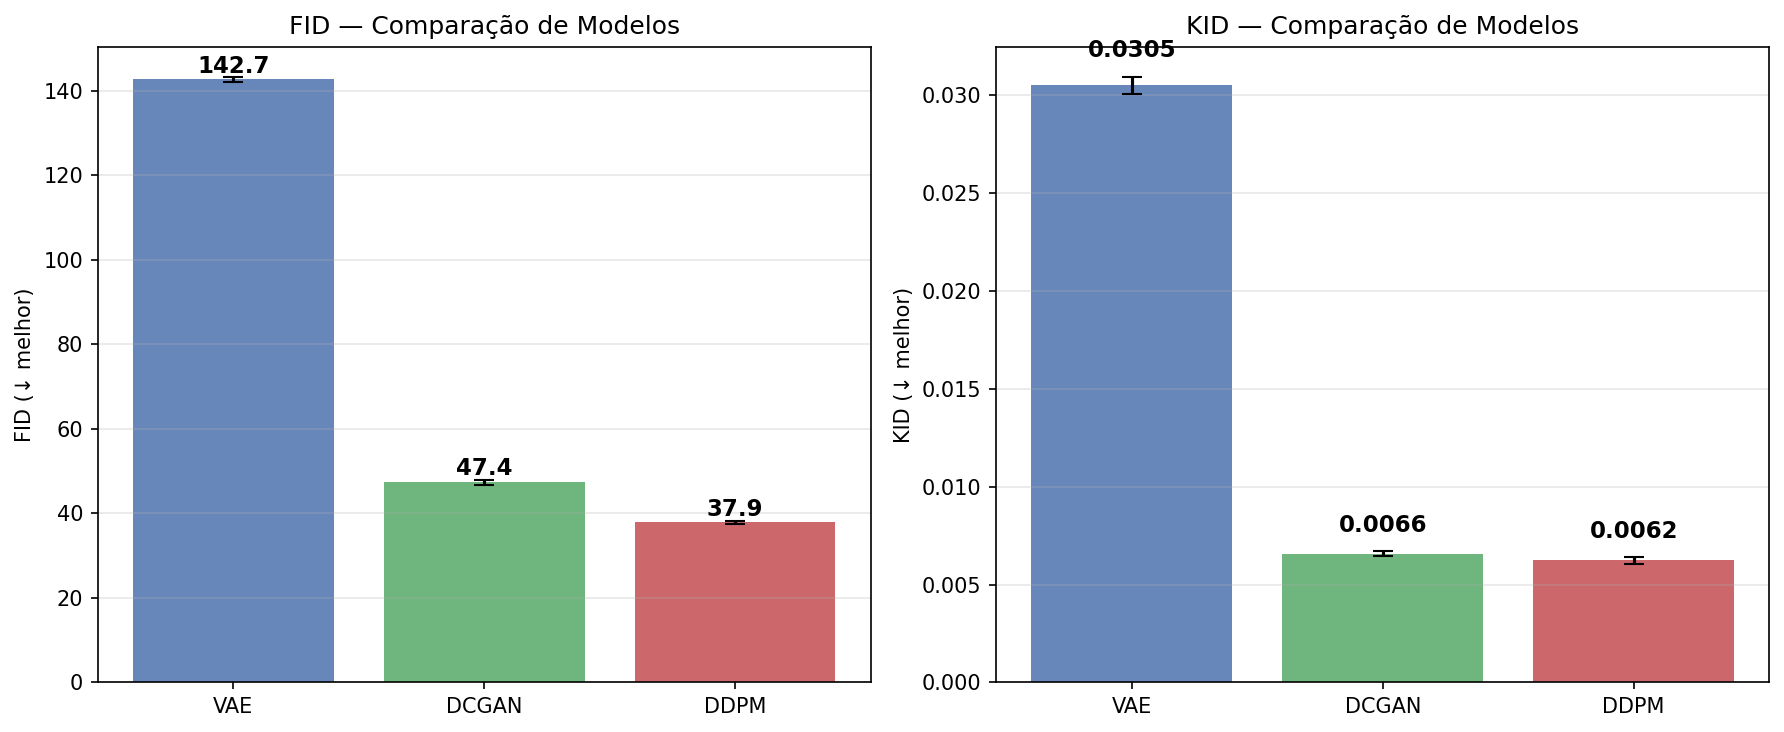
\includegraphics[width=0.90\textwidth]{comparacao_fid_kid.png}
  \caption{FID and KID on the 20\% subset (10 seeds, error bars = 1 std).}
  \label{fig:eval20}
\end{figure}

\FloatBarrier

On the subset, DDPM achieved a marginally lower FID ($45.91$) than DCGAN
($47.38$), while DCGAN led on KID ($0.0066$ vs.\ $0.0078$). The VAE lagged
by a wide margin ($142.72$). The near-parity between DCGAN and DDPM
motivated retraining both on the full dataset.

% ══ 6. PHASE 2: FULL DATASET ══════════════════════════════════════════════════
\section{Phase 2 --- Full Dataset (100\%)}
\label{sec:phase2}

All three models were retrained from scratch on the complete 50,000-image
training set with identical hyperparameters to Phase~1.

\subsection{VAE --- Full Dataset}

Figure~\ref{fig:vae100} shows VAE training curves and samples on the full
dataset. The total loss converged from~${\approx}1840$ to~${\approx}1780$
over 100 epochs, with the KL term stabilising at~${\approx}65$.
The 5$\times$ data increase did not qualitatively improve image sharpness,
confirming that blurriness is a structural limitation of BCE reconstruction
rather than a data-quantity issue.

\begin{figure}[!htbp]
  \centering
  \includegraphics[width=0.36\textwidth]{\imgVAEhundred}\hfill
  \includegraphics[width=0.61\textwidth]{\imgLossVAEhundred}
  \caption{VAE on full dataset. Left: 64 generated samples.
           Right: training curves (total loss, BCE, KL divergence).}
  \label{fig:vae100}
\end{figure}

\subsection{DCGAN --- Full Dataset}

Figure~\ref{fig:gan100} shows DCGAN results on the full dataset. Adversarial
losses maintained stable dynamics across 200 epochs. Sample quality improved
noticeably compared to Phase~1: images show richer colour palettes and finer
texture detail, consistent with the discriminator having access to 5$\times$
more real examples against which to sharpen the generator.

\begin{figure}[H]
  \centering
  \includegraphics[width=0.36\textwidth]{\imgGANhundred}\hfill
  \includegraphics[width=0.61\textwidth]{\imgLossGANhundred}
  \caption{DCGAN on full dataset. Left: 64 generated samples.
           Right: generator and discriminator loss curves.}
  \label{fig:gan100}
\end{figure}

\subsection{DDPM --- Full Dataset}

Figure~\ref{fig:ddpm100} shows DDPM results on the full dataset. The MSE
loss converged smoothly over 500 epochs with the warmup+cosine schedule.
Samples retain the high style diversity seen in Phase~1 and show further
improvement in colour coherence. However, the FID improvement from Phase~1
to Phase~2 was smaller than for DCGAN, suggesting the adversarial objective
is more sensitive to data quantity at $32\times32$ resolution.

\begin{figure}[H]
  \centering
  \includegraphics[width=0.36\textwidth]{\imgDDPMhundred}\hfill
  \includegraphics[width=0.61\textwidth]{\imgLossDDPMhundred}
  \caption{DDPM on full dataset. Left: 64 generated samples (DDIM, 100
           steps). Right: MSE loss and LR schedule over 500 epochs.}
  \label{fig:ddpm100}
\end{figure}

\subsection{Quantitative Evaluation --- Full Dataset}

Table~\ref{tab:results100} summarises the main results;
Table~\ref{tab:seeds} provides the full per-seed breakdown;
Figure~\ref{fig:eval100} visualises the distributions.

\begin{table}[!htbp]
\centering
\caption{FID and KID on the full dataset (mean~$\pm$~std, 10 seeds).
         Bold: best value.}
\label{tab:results100}
\begin{tabular}{lcc}
\toprule
\textbf{Model} & \textbf{FID} ($\downarrow$) & \textbf{KID} ($\downarrow$) \\
\midrule
VAE   & $140.37 \pm 0.43$ & $0.0314 \pm 0.0004$ \\
DCGAN & $\mathbf{30.46 \pm 0.57}$ & $\mathbf{0.0032 \pm 0.0001}$ \\
DDPM  & $37.91  \pm 0.37$ & $0.0062 \pm 0.0002$ \\
\bottomrule
\end{tabular}
\end{table}

\begin{table}[!htbp]
\centering
\caption{Per-seed FID and KID for all models (full dataset, seeds 42--51).}
\label{tab:seeds}
\setlength{\tabcolsep}{4.5pt}
\begin{tabular}{c rrr rrr}
\toprule
& \multicolumn{3}{c}{\textbf{FID}} & \multicolumn{3}{c}{\textbf{KID}} \\
\cmidrule(lr){2-4}\cmidrule(lr){5-7}
\textbf{Seed} & VAE & DCGAN & DDPM & VAE & DCGAN & DDPM \\
\midrule
42 & 140.66 & 31.10 & 37.91 & 0.0315 & 0.0032 & 0.0061 \\
43 & 140.34 & 29.56 & 38.35 & 0.0315 & 0.0033 & 0.0065 \\
44 & 139.59 & 29.91 & 37.63 & 0.0311 & 0.0031 & 0.0063 \\
45 & 140.29 & 30.29 & 37.88 & 0.0315 & 0.0032 & 0.0063 \\
46 & 140.34 & 30.23 & 38.05 & 0.0306 & 0.0032 & 0.0063 \\
47 & 141.28 & 31.35 & 37.39 & 0.0321 & 0.0033 & 0.0059 \\
48 & 140.76 & 30.87 & 38.29 & 0.0315 & 0.0034 & 0.0063 \\
49 & 140.07 & 30.70 & 37.20 & 0.0314 & 0.0032 & 0.0060 \\
50 & 140.26 & 29.73 & 38.04 & 0.0319 & 0.0030 & 0.0062 \\
51 & 140.08 & 30.82 & 38.33 & 0.0311 & 0.0032 & 0.0062 \\
\midrule
\textbf{Mean} & 140.37 & 30.46 & 37.91 & 0.0314 & 0.0032 & 0.0062 \\
\textbf{Std}  & 0.43   & 0.57  & 0.37  & 0.0004 & 0.0001 & 0.0002 \\
\bottomrule
\end{tabular}
\end{table}

\begin{figure}[H]
  \centering
  \includegraphics[width=\textwidth]{\imgMetricsHundred}
  \caption{FID (left) and KID (right) for all models on the full dataset.
           Error bars represent one standard deviation over 10 seeds.}
  \label{fig:eval100}
\end{figure}

\textbf{VAE.} The high FID ($140.37$) reflects the known limitation of
pixel-wise BCE: minimising average reconstruction error encourages blurry
outputs. The regularised latent space supports smooth interpolation but
does not enforce perceptual sharpness.

\textbf{DCGAN.} The adversarial objective directly minimises the perceptual
distance between real and generated distributions, yielding the best FID
($30.46$) and KID ($0.0032$). At $32\times32$ resolution the discriminator
has sufficient capacity to model the full feature space. The slightly larger
FID variance ($\pm0.57$) reflects GAN training stochasticity. Mode dropping
is qualitatively visible but not captured by FID/KID.

\textbf{DDPM.} The DDPM ranks second (FID~$37.91$) with the lowest variance
($\pm0.37$), indicating the most stable generation. The DDIM approximation
(100 vs.\ 1,000 steps) likely accounts for part of the gap with DCGAN.
At higher resolutions diffusion models typically surpass GANs~\cite{dhariwal2021};
at $32\times32$ the DCGAN's simpler objective is sufficient.

\subsection{Phase 1 vs.\ Phase 2 --- Cross-Phase Comparison}

Table~\ref{tab:comparison} quantifies the FID improvement from 20\% to
100\% training data.

\begin{table}[H]
\centering
\caption{FID improvement from Phase~1 (20\% subset) to Phase~2 (full
         dataset). $\Delta\text{FID}=\text{FID}_{100\%}-\text{FID}_{20\%}$.}
\label{tab:comparison}
\begin{tabular}{lccc}
\toprule
\textbf{Model} & \textbf{FID (20\%)} & \textbf{FID (100\%)}
               & $\boldsymbol{\Delta}$\textbf{FID} \\
\midrule
VAE   & $142.72$ & $140.37$ & $-2.4$ \\
DCGAN & $47.38$  & $30.46$  & $-16.9$ \\
DDPM  & $45.91$  & $37.91$  & $-8.0$ \\
\bottomrule
\end{tabular}
\end{table}

DCGAN benefited most from additional data ($\Delta\text{FID}=-16.9$),
followed by DDPM ($-8.0$). The VAE showed negligible improvement ($-2.4$),
confirming that its blurriness is a fundamental structural limitation rather
than a data-quantity issue.

% ══ 7. CONCLUSION ═════════════════════════════════════════════════════════════
\section{Conclusion}
\label{sec:conclusion}

We implemented and compared VAE, DCGAN, and DDPM on the ArtBench-10 dataset
under a rigorous two-phase protocol. The DCGAN achieved the best quantitative
results on the full dataset (FID~$30.46$), benefiting most from the larger
training set ($\Delta\text{FID}=-16.9$). The DDPM ranked second
(FID~$37.91$) with the lowest variance and greatest sample diversity,
while showing a moderate response to additional data ($\Delta\text{FID}=-8.0$).
The VAE ranked last in both phases, confirming that blur from BCE loss is
independent of dataset size.

These results highlight a key trade-off: at $32\times32$ resolution,
adversarial models excel at distribution matching, while diffusion models
offer richer diversity and are expected to scale better to higher
resolutions~\cite{rombach2022}. Future work includes full 1,000-step DDPM
sampling, class-conditional generation, and evaluation at higher resolutions.

\smallskip\noindent\textbf{Use of Generative AI Tools.}
Generative AI Tools like Claude, Gemini and
Chat GPT were used as a code assistant during the development of this project,
specifically to help structure training loops, debug PyTorch code, and draft parts
of this report. All model implementations, experimental results, and conclusions
were verified by the authors.

% ══ REFERENCES ════════════════════════════════════════════════════════════════
\begin{thebibliography}{10}

\bibitem{dhariwal2021}
Dhariwal, P., Nichol, A.: Diffusion models beat GANs on image synthesis.
In: Advances in Neural Information Processing Systems (NeurIPS) (2021)

\bibitem{gulrajani2017}
Gulrajani, I., Ahmed, F., Arjovsky, M., Dumoulin, V., Courville, A.C.:
Improved training of Wasserstein GANs.
In: Advances in Neural Information Processing Systems (NeurIPS) (2017)

\bibitem{ho2020}
Ho, J., Jain, A., Abbeel, P.: Denoising diffusion probabilistic models.
In: Advances in Neural Information Processing Systems (NeurIPS) (2020)

\bibitem{karras2020}
Karras, T., Aittala, M., Laine, S., H{\"a}rk{\"o}nen, E., Hellsten, J.,
Lehtinen, J., Aila, T.: Training generative adversarial networks with limited
data. arXiv preprint arXiv:2006.06676 (2020)

\bibitem{karras2018}
Karras, T., Laine, S., Aila, T.: A style-based generator architecture for
generative adversarial networks. arXiv preprint arXiv:1812.04948 (2018)

\bibitem{kingma2013}
Kingma, D.P., Welling, M.: Auto-encoding variational Bayes.
arXiv preprint arXiv:1312.6114 (2013)

\bibitem{liao2022}
Liao, P., Li, X., Liu, X., Keutzer, K.: The ArtBench dataset: Benchmarking
generative models with artworks. arXiv preprint arXiv:2206.11404 (2022)

\bibitem{radford2015}
Radford, A., Metz, L., Chintala, S.: Unsupervised representation learning with
deep convolutional generative adversarial networks.
arXiv preprint arXiv:1511.06434 (2015)

\bibitem{rombach2022}
Rombach, R., Blattmann, A., Lorenz, D., Esser, P., Ommer, B.:
High-resolution image synthesis with latent diffusion models.
In: IEEE/CVF Conference on Computer Vision and Pattern Recognition (CVPR) (2022)

\bibitem{sohn2015}
Sohn, K., Lee, H., Yan, X.: Learning structured output representation using
deep conditional generative models.
arXiv preprint arXiv:1506.05517 (2015)

\end{thebibliography}

\end{document}
